\documentclass[twocolumn]{article}
\pagestyle{empty}
\setlength{\textwidth}{7in}
\setlength{\textheight}{9.125in}
\setlength{\columnsep}{0.5in}
\setlength{\topmargin}{-0.8in}
\setlength{\oddsidemargin}{-0.25in}
\setlength{\parindent}{5 ex}
 
\usepackage[numbers]{natbib}
\renewcommand{\bibfont}{\footnotesize}% set bibliography font to small

\usepackage{epsfig}
\usepackage{subfigure}
\usepackage{algorithm}
\usepackage{algorithmic}	
\usepackage{calc}
\usepackage{amssymb}
\usepackage{amstext}
\usepackage{amsmath}
\usepackage{amsthm}
\usepackage{eqparbox}

\makeatletter
\def\@normalsize{\@setsize\normalsize{12pt}\xpt\@xpt \abovedisplayskip 11pt
plus2pt minus5pt\belowdisplayskip \abovedisplayskip \abovedisplayshortskip \z@
plus3pt\belowdisplayshortskip 6pt plus3pt
minus3pt\let\@listi\@listI}
%the following line was changed
\def\subsize{\@setsize\subsize{12pt}\xipt\@xipt}
\def\section{\@startsection{section}{1}{\z@}{24pt plus 2 pt
minus 2 pt} {12pt plus 2pt minus 2pt}{\large\bf}}
\def\subsection{\@startsection {subsection}{2}{\z@}{12pt
plus 2pt minus 2pt}{12pt plus 2pt minus 2pt}{\subsize\bf}}
\makeatother
\begin{document}
\date{}
\title{\Large\bf Reconstruction of Fine Level Geometric Structure From Stereo Pairs in the Underwater Setting}
%\author{I. M. Author \\
%My Department\\
%My Institute \\
%My City, ST, Zip}
%for two authors (type the following)
\author{\begin{tabular}[t]{c@{\extracolsep{8em}}c}
I. M. Author & U. R. Coauthor \\
My Department & Coauthor Department\\
My Institute & Coauthor Institute \\
City, St ~~Zip & City, ST~~Zip
\end{tabular}}
\maketitle
\thispagestyle{empty}


\subsection*{\centering Abstract}
\vspace*{-3mm}
The study of underwater structures, such as wells, cisterns, and water storage systems, can be of historical and scientific significance for archeologists. However, access to and study of such sites can be dangerous or infeasible for humans. Underwater micro-ROVs, such as the VideoRay Pro III GTO, can often reach and navigate these locations safely while causing less harm to the site. Prior work has successfully reconstructed geometric models of such underwater structures with the use of sonar measurements. Although effective, sonar has a limited resolution and omits many fine geometric details of the model in the scanning process. In this paper, we present a preliminary solution towards the reconstruction of fine details of geometric features in the underwater setting using stereo pairs. These fine details can then be integrated into 3D models reconstructed from sonar to create a more visually accurate model. We present initial results and detailed methodology for future data acquisition.
\\
\\
\noindent {\bf Keywords:} 5 KEY WORDS HERE

\section{Introduction}
Recent research in the field of mobile robotics has demonstrated the creation of 3D maps of settings otherwise inaccessible to humans, such as narrow tunnels and marine caves~\cite{ICEX11,McVicker}. Progress made in Simultaneous Localization and Mapping (SLAM) algorithms  (\cite{Williams2000},~\cite{harbor}, and \cite{Fairfield2006}) allow robots to localize themselves and create these maps using input from sonar, infrared, and other scanning sensors. Such maps, or evidence grids, can then be treated as implicit volumes and then used to construct a geometric model of the scanned regions using marching cubes~\cite{Lorensen}. An example of a geometric model of a well used for water storage can be seen in Figure~\ref{fig:wellNoFine}. Unfortunately, equipment limitations, sensor noise, and probabilistic uncertainty occurring in the data acquisition process cause these models to suffer from a loss of fine geometric details. Loss of detail in the scanning process is a problem for end-users, who wish to study these models or use them for educational purposes. In this paper we present a preliminary solution towards the reintroduction of fine details omitted by sonar data into surface reconstructions via the use of two cameras to capture stereo images of underwater surfaces.  The stereo images are then processed to produce disparity maps which contain the fine geometric detail of the original surface. The depth information in each disparity map can then be used to enhance the final geometric model.

This project is a part of a larger ongoing project, with the broad goal of mapping and modeling ancient water storage systems, i.e. cisterns, wells and water galleries located in most houses, churches, and fortresses on the islands of Malta, Gozo, and Sicily. This multiple year project involves the deployment of a micro-ROV into water systems in the Mediterranean~\cite{White10,ICEX11,McVicker} with this paper documenting the first use of stereo data for fine level geometry acquisition. The data used in this paper was gathered through a series of underwater robot deployments in which multiple sonar scans were gathered, then fused into a map of the scene via SLAM algorithms. In addition to the sonar data, stereo pairs were obtained for use in creating disparity maps to model fine level geometry. 
%In order to annex this fine geometry to the general models, both the color data and disparity information from the disparity maps are projected onto the geometric model generated from the sonar data via projective texturing. Finally, the geometry contained within the frustums of the projectors in the model is displaced in accordance with the projected disparity maps, preserving the fine details omitted in earlier stages of reconstruction. 
The stages of our algorithm can be seen in Figure~\ref{fig:systemblock}.

%The results reported in this paper are from preliminary work in a multidisciplinary setting, utilizing aspects of emerging robotics and computer graphics technology. 
The goal of this work is the generation of a computer model which includes the fine organic features found in underwater storage systems.
This paper outlines the data acquisition and stereo displacement map computation, describes our solution to displacing rough geometry in accordance with a projected disparity map, illustrates our results on a model using a partial  data set, and outlines a data acquisition process for future missions. 

\begin{figure*}[!ht]
  \vspace{-0.2cm}
  \centering{
     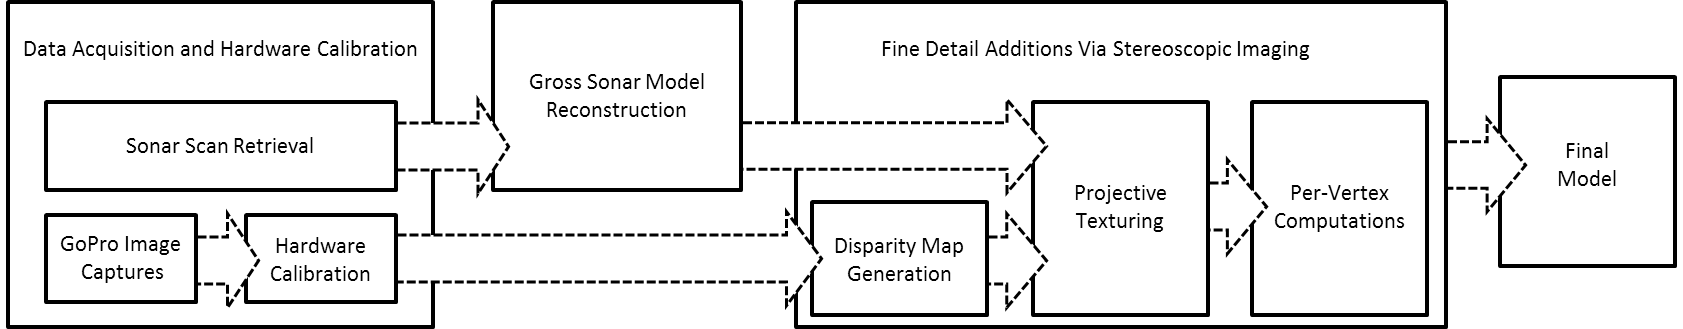
\epsfig{file = pics/systemBlock.png, width = \textwidth}}
  \caption{The pipeline used to add fine details to a sonar generated mesh.}
 \label{fig:systemblock}
\end{figure*}

%There is 1 blank line before the section heading and one afterwards. Heading text is 11 point bold font.
%You may cite references of the form \cite{key:foo} or \cite{foo:bar}, andLaTex will keep track of numbering. The numbers are based on the order you place them in the bibliography, not the order they appear in the text. They should be in alphabetical order. LaTex will put square brackets around the number in the text of your paper. You must run the latex process twice to allow the references to format properly. You will see a message about a missing .aux file. Simply latex it a second time and it will be fine.
\section{Related Work}
\label{sec:data}
This project relies on data acquired from algorithms for mapping with underwater robots (e.g.~\cite{Williams09},~\cite{opizarro-2009a},~\cite{Fairfield2006},~\cite{Clark2008b}). For a good survey of the core techniques capable of fusing data from multiple sensors, see Thurn~\cite{Thrun2005}.
For this project the most relevant  research in underwater robot Simultaneous Localization and Mapping (SLAM) is found in (e.g.~\cite{Williams2000},~\cite{harbor}, and~\cite{Fairfield2005,Fairfield2006}).
%TP: move somewhere else?
Related work in stereo vision based SLAM algorithms has been performed to generate 3D maps of the seafloor~\cite{Mahon:2011},~\cite{stereo:Roberson}.

In addition, this work relies on well known algorithms from computer graphics, such as surface extraction from volume data using marching cubes~\cite{Lorensen}, projective texturing and texture mapping~\cite{Williams78castingcurved,Segal}, and the use of vertex shaders to displace existing vertices on the GPU. Work in~\cite{Fairfield:2010} likewise uses marching cubes to create a geometric model of underwater structures from an evidence grid, but uses a far more complex ROV with extensive sensors.

This research relies on related work in the field of stereoscopic data acquisition and disparity map reconstruction~\cite{stereo:gutMarroquin},~\cite{stereo:scharsteinSzeliski}.
In particular, this work uses the method of~\cite{stereo:zitKan} to generate disparity maps from underwater stereo image pairs.
The work of~\cite{stereo:nalGast} was also explored to allow us to avoid comparing the differences in light intensities between images.
We found, however, that the underwater setting does not transmit colors well, which forced us to return to using differences in light intensities.
\vspace{-11pt}
\section{Data Acquisition}
\label{sec:data}

A VideoRay Pro III GTO micro submersible Remotely Operated Vehicle (ROV) is utilized in the data acquisition process (Figure~\ref{fig:ROV}). 
%The ROV is deployed into a cistern and guided from a control module above the surface. 
During deployment, the navigator repeatedly rests the ROV on the cistern floor and records a $360^{\circ}$ stationary sonar scan, then the ROV is repositioned in the cistern for another scan to collect an entire horizontal scan. 
%The sonar scans must have some overlap to facilitate mosaicing and localization for surface reconstruction, which is taken into consideration when positioning the ROV on the cistern floor. The approximate position and heading of the ROV is recorded before each scan for later use in aligning projectors in the geometric model. The ROV's main video camera is used to position the unit at each location. 
A more complete overview of the sonar data acquisition process can be found in~\cite{ClarkVast}. This collection of sonar scan planes is then used to build a general 3D model of the cistern~\cite{ICEX11}.

While the sonar scans are being collected, the ROV captures stereo image pairs of the cistern walls. These images are collected using two GoPro HD Hero2 cameras mounted to the front of the ROV, which are synchronized through the 3D Hero System waterproof housing and connector cable. The default domed lenses of the 3D Hero Housing distort images taken underwater, so flat lenses were installed to minimize complexity during data processing. The camera unit is unable to be controlled remotely, and instead, each camera is set to capture an image every second. To collect stereoscopic images the ROV is maneuvered around the edges of the cistern, pausing every few feet. The ROV is positioned roughly one meter from the wall to capture stereo pairs with features that can be easily matched later. The images captured at each of these locations are used to create disparity maps, as described in Section~\ref{disparityMapGeneration}.

\begin{figure}[!h]
   \vspace{-0.2cm}
   \centering{
      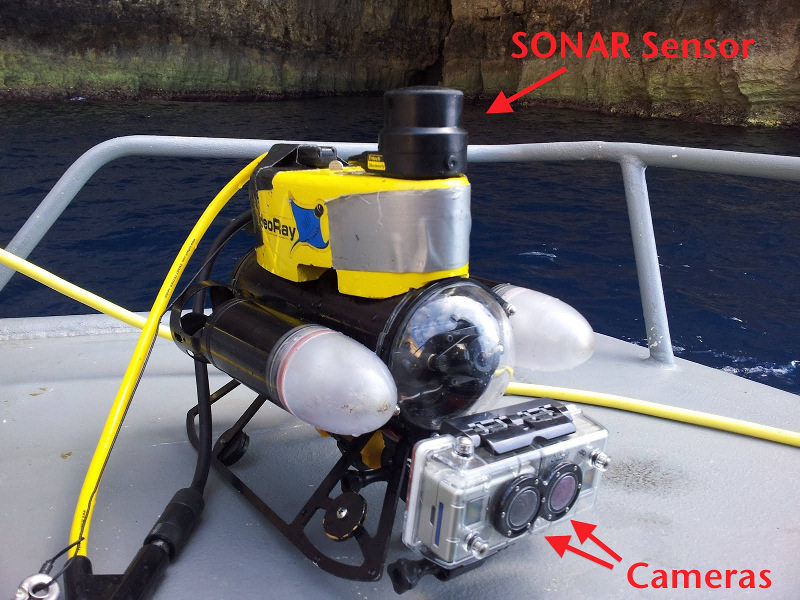
\epsfig{file = pics/ROV.jpg, width = 6cm}}
   \caption{Hardware setup: Tritech SeaSprite sonar sensor, 2 vertically aligned GoPro HD Hero2 cameras mounted on a VideoRay Pro III GTO micro ROV.}
  \label{fig:ROV}
 \end{figure}

\paragraph{Hardware Calibration}
% HAVE NOT EDITED YET
To facilitate the virtual reconstruction of the world it was necessary to calibrate the GoPro cameras.
Both the aspect ratio and the vertical field of view (VFOV) needed to be calculated to accurately re-project the captured images and disparity maps in the virtual world.  
The following equations were used:
\vspace{-11pt}
\begin{align}
\text{aspect ratio} &= \frac{\text{width}}{\text{height}} \\
\text{VFOV} &= 2\tan^{-1}\left({\frac{\text{height}}{2\text{depth}}}\right)
\end{align}
These two values were used to specify the behavior of projectors, discussed later in Section~\ref{subsec:projectiveTexturing}.

\paragraph{Gross sonar Model Reconstruction}
\label{sec:reconstruction}
Prior work is focused on reconstructing general geometric models from evidence maps representing Mediterranean water storage systems (cisterns, wells and water galleries)~\cite{ICEX11,McVicker}. As a pre-process to the algorithms presented here for fine level geometry modeling, the cisterns are mapped using sonar data, which is fused into a two dimensional grid of cells with a likelihood $p_{i,j} \in [0,1]$ of being occupied \cite{Thrun2005} and~\cite{White10}. This single 2D layer can then be extruded into a 3D evidence grid and treated as volume data. A polygonal geometric model of the scanned data can be constructed via marching cubes, where any cell with $p_{i,j}$ greater than a threshold value, $t$, is considered an occupied cell and associated with a wall in the model. $t$ is used to define occupancy and is generally set to values in the range $.65-.85$. We refer the reader to~\cite{ICEX11,McVicker} for more details on the mapping process.

%\section{\uppercase{Fine Detail Additions Via Stereoscopic Depth Extraction}}
\section{Constructing a more accurate geometric model}
\label{sec:detail}

\noindent The models constructed from the evidence grid give a good representation of the gross shape of an underwater system. However, due to challenges in the acquisition process for sonar data, these models tend to lose the fine geometric details present in many of the mapped structures, which are important to archaeologists seeking to study the underwater system. See Figure~\ref{fig:wellNoFine} for an example of a well model constructed from sonar data alone. In contrast, Figure~\ref{fig:disparity} shows a photograph of the side of the well, where it is clear that fine level details such as the rocks that comprise the walls are not well modeled by the sonar reconstruction alone.

%The first step towards building fine details into a planar mesh is extracting those details from the original surface. We used stereo vision. 
To capture fine details, pairs of stereo images (left and right images of the same surface) were compared to form a disparity map and to capture the color data of the surface walls.
Due to hardware constraints, our stereo setup is only accurate for determining the distance of objects up to two meters away from the cameras.
This constraint was not an issue for our purposes, as the ROV was held roughly one meter from the wall when capturing images.

To integrate these fine details into the exisiting geometric model requires the use of the disparity maps and image pairs to deform and texture, respectively, the basic sonar mesh.
There are two challenges at this stage in the process.  One is accurately localizing the ROV with respect to the general model to correctly project the disparity maps onto the model surface. The second is mapping captured depth information onto the existing model.
For the current implementation, we do not include a computational solution to the first challenge. 
Instead, the preliminary results presented in this paper are from a cylindrical well with rotational symmetry and a user interactively sets the location from which data was acquired.

The second challenge is resolved by using the pixel intensity data stored in the grayscale disparity map to deform the vertices onto which the disparity map was projected.
Light patches of the disparity map pull vertices towards the projector and away from the existing wall, while dark patches push those vertices into the wall.
One of the two stereo images is projected onto the deformed model, giving the model both the color and shape of the original surface. Repeating this procedure for each section of wall produces a finely detailed 3D model of the cistern.

\begin{figure}[!h]
	\centering
		\subfigure[Well Top View]{\label{welltop}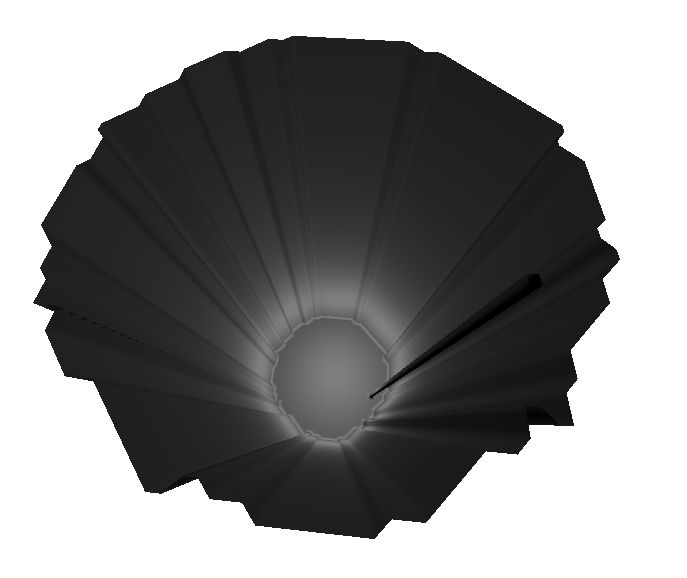
\epsfig{file = pics/cisternTop.png, width = 3.5cm}}
		\quad %space between images
		\subfigure[Well Side View]{\label{wellside}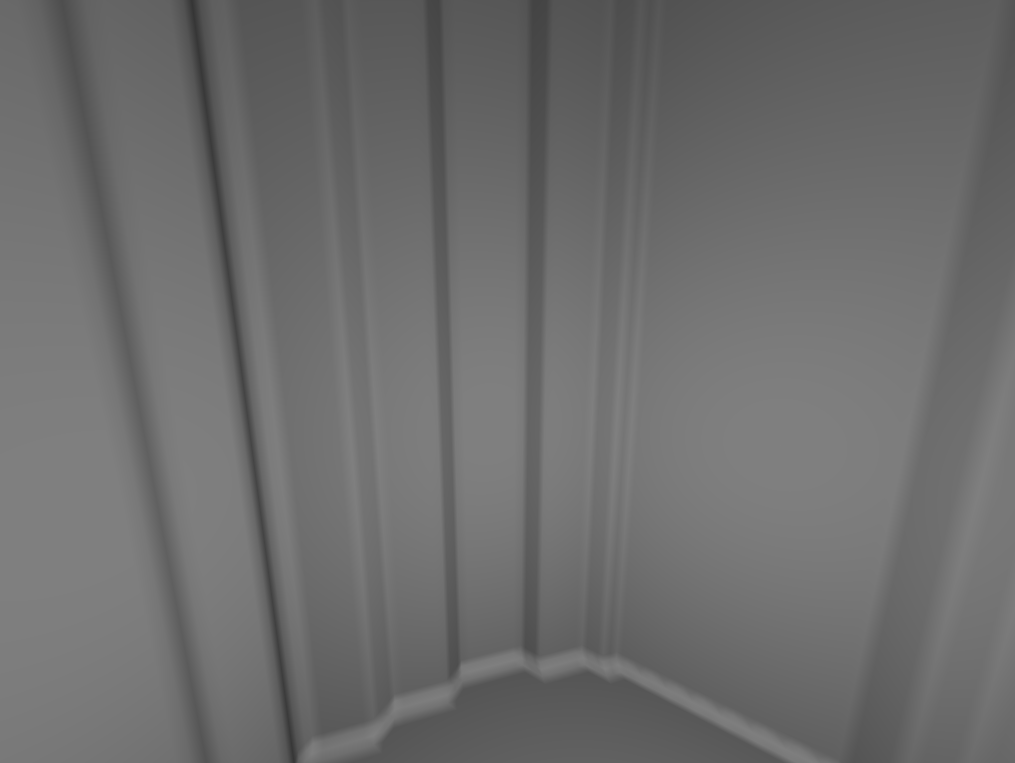
\epsfig{file = pics/cisternWall.png, width = 3.5cm}}\\%new line

		\caption{Views of Plain Well Geometry}
		\label{fig:wellNoFine}
\end{figure}

%\begin{figure}[!h]
%	\centering
%		\subfigure[Well Photo]{\label{right}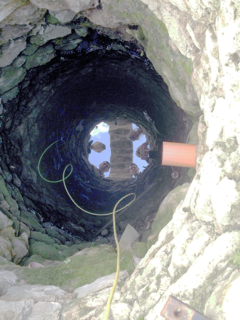
\epsfig{file = pics/wellPhoto, width = 3.5cm}}\\%new line

%		\caption{ A photograph of the walls of the well.}
%		\label{fig:wellPhoto}
%\end{figure}

\subsection{Disparity Map Generation}
%{ HAVE NOT EDITED YET}
\label{disparityMapGeneration}

A number of stereo vision algorithms currently exist to compare the features of two images in order to determine the distance between the feature and the camera.
% few of these algorithms are robust enough to handle compressed underwater images of rock walls combined with poor lighting conditions and very shallow features.
However, rocks and bricks, two common features found on cistern walls, have highly repetitive patterns and colors--providing only a few unique features.  In addition, the images  captured within the cisterns usually contain poor lighting, and shallow depressions (in comparison to images with large color or depth contrast).  All of which prove to be challenging to most stereo vision algorithms.
After exploring several options, the stereo mapping algorithm described by Zitnick and Kanade in~\cite{stereo:zitKan} was chosen for the current implementation.

Most stereo-matching algorithms, including Zitnic and Kanade, rely on unique features between images to aid in pixel mapping.
Specifically, the algorithm proposed by Zitnick and Kanade uses a scanning, sliding comparison window to build an initial disparity map.
To mitigate the dull landscape, we choose a large initial comparison window with a radius of five pixels.
This decision reduces the level of fine details that can be resolved from the image and adds a smoothing effect to the disparity map, but these drawbacks are acceptable in the given environment.
Instead, a large window gives a more reliable matching between rocks faces because it encompasses more features for each pixel.  

Lighting was perhaps our most challenging issue. 
Most of the water systems explored were dark (with very little light entering the systems through narrow tunnels and openings).
Meaning that the imaged surfaces were lit almost solely by the ROV's onboard lights and that the ROV had to fly relatively close to the walls in order to illuminate features for the cameras.
Each camera computed its own exposure time based on the amount of light it received.  
As a result of some well illuminated features being closer to one camera than the other, there are discrepancies in exposure times between left and right images, (see Figure~\ref{fig:disparity} for an example of this contrasting lighting).
We attempted to use the work in \cite{stereo:nalGast} to fix this problem by shifting the image into the HSL color space.  For our purposes, however, this method failed since too much of the color from our ROV's lights was absorbed by the water to allow us to use images in the HSL space.

Another common challenge is the presence of dirt particles in the images.
This is due to the ROV's positioning thrusters agitating sediment in the water systems.
Usually the particles are small enough to be detected as occlusions and removed from the final disparity map by the Zitnick and Kanade algorithm.

\begin{figure}[!h]
	\centering
		\subfigure[Left image]{\label{camleft}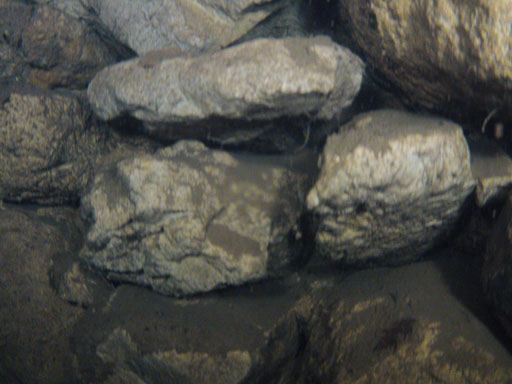
\epsfig{file = pics/372L.jpg, width = 3cm}}
		\quad %space between images
		\subfigure[Right image]{\label{camright}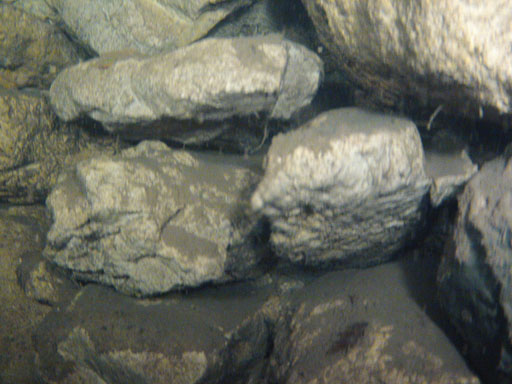
\epsfig{file = pics/372R.jpg, width = 3cm}}\\%new line
		\medskip
		\subfigure[Generated Disparity Map]{\label{disparitymap}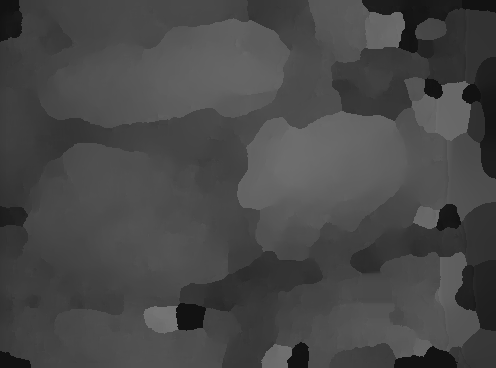
\epsfig{file = pics/372disp.png, width = 5cm}}
		\caption{An example disparity map generated with initial local support region of (13,13,5), and an iterative support region of (11,11,5).}
		\label{fig:disparity}
\end{figure}

\paragraph{Image Correction}
% HAVE NOT EDITED YET}
%\label{subsec:image_correction}

In many stereo mapping algorithms, including Zitnick and Kanade, it is assumed that both images are accurate down to the pixel level.
Regrettably, the GoPro cameras used were limited to recording images in the lossy .jpeg format only.
To solve this issue we smoothed and shrunk the high resolution .jpeg images taken by the GoPros to produce smaller left and right images that were comparable at the pixel level.

Image correction starts with a smoothing step.
  A simple Gaussian smoothing step was ineffective in this case because it blurred the edges of the rocks or bricks, removing valuable features from an already feature-scarce image.
  Instead an image smoothing tool was used (Photoshop's "surface smooth") which preserved edges while still blurring similar color regions.
  Next a shrinking step was performed on the image to further reduce artifacts and trim the size (from 3200 by 2400 to 512 by 384).
The final size was large enough to preserve the details in the image, while still providing a significant size reduction to artifacts.   
%Through experimentation, we discovered that the best image detail to process time ratio was obtained by reducing the images by one sixth.   
%Shrinking was performed after smoothing to preserve the maximum amount of detail in the image.

Similar to the work of Johnson-Roberson, we explored accounting for illumination fade-off, or vignetting, across our image sets (~\cite{stereo:Roberson}).  
We found, however, that due to our close proximity to walls and narrow field of view, de-vignetting our images had little effect.

\paragraph{Disparity Mapping}
% HAVE NOT EDITED YET}
%\label{subsec:disparity_mapping}

Disparity maps were generated using the cooperative, iterative approach described by Zitnick and Kanade~\cite{stereo:zitKan}.
The basic algorithm is as follows:
\begin{itemize}
\item Find the local support for each pixel at $(x,y)$ and each depth, $d$, by using an image intensity comparison function, $\delta$.
We chose $\delta$ to be a normalized correlation function.
\begin{equation}
L_0(x,y,d) = \delta(I_{Left}(y,x),I_{Right}(y,x+d))
\end{equation}
\item Copy the values from the 3D array $L_0$ into a new 3D array, $L_n$.
\item Assume that $\Phi(x,y,d)$ is the 3D support region around the pixel $(x,y)$, and suppose
\begin{equation}
S_n(x,y,d) = \hspace{-14pt} \sum_{(x',y',d') \in \Phi} \hspace{-14pt} L_n (x+x', y+y', d+d')
\end{equation}
Furthermore, assume that $\Psi(x,y,d)$ is the set of all pixels that map to $(x,y)$ in the left image and $(x+d,y)$ in the right image. 
Let $\alpha$ be a constant that controls how quickly the values in $L_n(x,y,d)$ will converge. Then, iterate through the values in $L_n$ updating each value using
\begin{align}
\nonumber
L_{n+1}(x,y,d) &= \\ 
\vspace{-10pt}
L_n(x,y,d)&\left(\frac{S_n(x,y,d)}{\sum\limits_{(x'',y'',d'') \in \Psi(x,y,d)} \hspace{-30pt} S_n(x'',y'',d'')} \right)^\alpha 
\end{align}
\item To build the final disparity map, loop through each pixel position $(x,y)$ and award the depth value $d$ with the highest weight from $L_n(x,y,d)$ as the final value.
If the best weight for all depths for a certain pixel $(x,y)$ is below a predefined threshold, assume the pixel was occluded.
\end{itemize}
%\subsubsection{Post Disparity Generation Correction}
%\label{subsec:post_zitcan_correction}

%All of the disparity maps generated by the Zitnick and Kanade algorithm had slight errors around the edges.  
%Patches of the image would either be unreasonably close to the camera or flat against the background.  
%These images had to be corrected before they could be mapped to vertices.  

\paragraph{Calibration}
% HAVE NOT EDITED}
%\label{subsec:calibration}

An important step in any meaningful recreation, including disparity mapping, is calibration.
This is the creation of a tuned mapping from a grayscale pixel value to the appropriate vertex offset in the virtual world.  
Pictures of a patterned surface were taken at a number of measured distances from that surface.
Those images were then disparity mapped, and the average disparity at the center of the picture was used as the disparity data point for that physical depth.
We used that set of points to create an exponential relationship between disparity value and physical depth.  
That equation is used later to accurately recreate the internal dimensions of the cistern, see section~\ref{vertexdisp} for more info.

%ZJW: Need a concluding paragraph about disparity map generation - Also should you say something about smoothing out spurrious data?
%TP: we could break the "smoothing" into its own section as is commented above... but for now it works here.
After the disparity maps were generated, a number of them had obvious errors--small regions of all white and all black.  
These erroneous regions were fixed by flooring and capping the intensity of the pixels. 
Pixels that had unreasonably small values were simply increased in value to a reasonable minimum, around 1.5 meters.  
Groups of pixels that were too large in value were deleted and replaced by a linear smoothing of the surrounding reasonable pixel values. 

Using the above described methods, the computed disparity maps are then used to provide depth values to displace the general geometry created from the sonar data. Figure~\ref{fig:disparity} illustrates a disparity map generated using our implementation.

\subsection{Projective Texturing}
\label{subsec:projectiveTexturing}

%ZJW: need to motivate projective texturing - please read what I wrote and edit as desired
\noindent In order to add fine details to the general mesh created from sonar data, $M_s$, we map the location of the disparity map data onto the global coordinates of the general mesh. Ideally, localization of the ROV's position could be computed and then used to correspond the coordinates of the general mesh and the displacements. With our current hardware, ROV localization is only computed for fixed scans and the ROV's position with respect to the map is unknown for each stereo pair capture. Future work includes using additional hardware such as a Smart Tether to assist in localization, but for our preliminary results, we use projective texturing with a user's input to manually align disparity map and image projections. In general, the onboard camera captures an image of an organic feature in a cistern, and our implementation allows the user to position a projector which casts the image from the same relative position onto the general mesh for displacement. Projective texturing is utilized because of its ability to properly simulate the onboard camera as a point particle with the camera's view frustum modeled as six implicit plane equations (i.e. modeling the camera field of view). Our implementation allows the projection of multiple textures and disparities, building a more detailed and colored model as more images and disparities are placed and added to the original mesh.

The combination of projective texturing and stereoscopic imaging enables our system to selectively displace vertices according to the color of a texture-mapped disparity map that is projected onto a surface. These vertices are displaced along the vector leading from their original 3D position in the mesh to the center of projection of the projector (or virtual camera). We used graphics libraries, OpenGL and OpenGL Shading Language (GLSL) to aid in projective texturing, the latter being used to create shaders - small programs run per-vertex or fragement directly on the GPU. The shaders are programmed to selectively alter rendered vertex position (vertex shader) and color (fragment shader).

A projector is simulated by establishing plane equations for a view frustum based on the position and orientation of the ROV's onboard camera when the projected images were captured in a cistern. We define $J = \{j_{1},\dots,j_{N}\}$ to be the set of projectors casting textures onto the gross surface reconstruction. Each projector, $j_{n} = (j_{n}^{pos}, j_{n}^{look})$, is uniquely defined by its position in 3D space, and a look vector orthonormal to the projector's viewport (Figure~\ref{fig:frustum}). All projectors have a pre-calibrated Field Of View (FOV) mimicking the compound FOV produced by the GoPro camera and waterproof housing lenses. The ROV is not equipped with roll thrusters, allowing us to ignore the possibility of a tilted camera frustum (i.e. the projector's right facing vector will always lie in the horizontal plane). Implicit plane equations modeling the projector view frustums in the form $Ax + By + Cz + D = 0$ are resolved using the clip space approach, where $\langle A, B, C\rangle$ is the plane's normal vector and  $(x, y, z)$ is a point on the plane. In this approach, plane equations for each projector are computed in homogenous space using the composite $4x4$ modelview projection matrix of the projector. See~\cite{vfc} for more information on the projective texturing implementation.

Each vertex, $p_{m}$, is defined by its position in 3D space and in order to limit the displacement to only vertices 'seen' by the curent projector, view-frustum culling was used. The full set of vertices contained in the mesh, $P$, is passed through a view frustum culling filter, yielding a set of vertices containing only those vertices in the frustum volume of one or more projectors, $P^*$ (Figure~\ref{fig:frustum}). Both $P$ and $P^*$ are sent to the shaders for per-vertex displacement computations.

\begin{figure}[!h]
   \vspace{-0.2cm}
   \centering{
      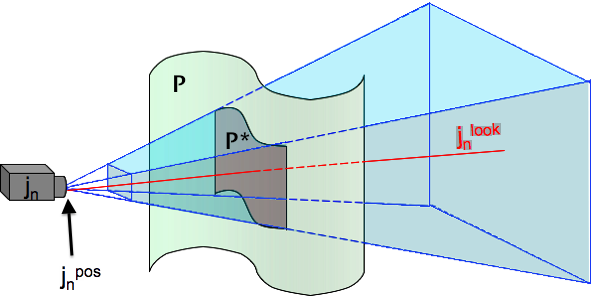
\epsfig{file = pics/frustum.png, width = 6cm}}
   \caption{Frustum and viewport.}
  \label{fig:frustum}
 \end{figure}

The implemented projective texturing method naturally produces a second projection facing in the direction negative to $j_{n}^{look}$. To remove the unwanted projections, a simple check was added to the vertex shader which ensures that the texture mapped vertex position has a positive $q$ component.

\subsection{Per-Vertex Displacement Computations}

A GLSL vertex and fragment shader are used to displace and texture vertices. The vertex shader recieves all of the vertices in the mesh, $P$, with vertices lying in the frustum of one or more projectors, $P^*$, marked. The vertex shader also recieves a modelview projection matrix for the camera and each projector, projector positions, texture primitives for the disparity maps, and offset distances from the wall for each texture from the CPU. The vertex shader displaces vertices one at a time in accordance with the color of the disparity map with respect to the texture-mapped coordinates. Vertices belonging to $P^{*}$ have their position updated. Vertices lying in the frustum of two or more projectors have their displacement vectors blended.

Since the vertex shader is run individually on each vertex, it does not have access to neighboring vertex information. Thus in order to correctly compute normal vectors of the displaced mesh for diffuse shading, the updated position of each vertex must be sent back to the CPU where the entire array of vertices can be accessed. Normals are recomputed for the displaced mesh, and updated normals as well as the displaced mesh are sent to a fragment shader. The displacement vertex shader is only used on the first render, after which time the displaced mesh and updated normals are used for every subsequent render.

The fragment shader receives $P$ and $P^{*}$, as well as the camera image texture primitives and the updated normals. The fragment shader maps the camera images onto the vertices in the frustum of each projector. Again, vertices lying in the frustum of two or more projectors have their colors blended. Once an RGB color value has been computed for the vertex, diffuse shading is added to the model using the updated normals.

\paragraph{Vertex Displacement}
%\label{sec:vertexdisp}

Vertices belonging to $P^{*}$ are displaced along the vector $\vec{b} = j_{n} - p_{m}$ a distance based on the RGB color value, $\vec{C} = \langle C_{r}, C_{b}, C_{g} \rangle$, of the disparity map at the corresponding texture-mapped coordinates, $t_m$. The texture-mapped coordinates of $p_m$, and thus, $\vec{C}$ can be calculated per-vertex using the modelview projection matrix of the projector by
\begin{align}
t_{m} &= p_{m}\lbrack MVP \rbrack _{j_{n}} \\
\vec{C} &= \langle t_{m\_red}, t_{m\_blue}, t_{m\_green} \rangle
\end{align}
The disparity map is greyscaled such that the disparity value is stored within each of the three members of $\vec{C}$, so only $C_r$ is required for distance computations. The disparity map contains disparity information rather than distance to the wall, so $\vec{C}$ is passed into an exponential equation obtained during calibration, $D(C_r)$, to resolve the true distance to the wall. $D(C_r)$ was computed by measuring known distances from the cameras to a checkerboard pattern, and fitting a least squares function to disparities obtained from the resulting stereo pair. The world space coordinates of $M_s$ are computed such that one unit in world space is equal to one meter in the cistern, so the value returned from passing $C_r \in [0, 1]$ into the distance function is the true wall distance in meters. With this in mind, vertex displacement proceeds as follows:
\begin{equation}
p_{m}' = \left \{ 
\begin{array}{ll}
p_{m} + (\vec{b} - D(C_r)\hat{b})  & \text{if} \quad p_{m} \in P^{*}\\
p_{m} & \text{otherwise}
\end{array},\right.
\label{eq:displace}
\end{equation}
where $p_{m}'$ is the displaced vertex position, with the calibrated distance function
\begin{equation}
D(C_r) = 1.547 e ^{-\left(0.018 * 255\right)C_r}
\end{equation}
 \paragraph{Projection Blending}

%Feel free to remove/edit/use for inspiration
The existence of multiple projectors in the model requires the ability to artfully and accurately overlap and blend projections. 
%Every projection has an equal likelihood of being the ground truth data for a vertex. 
%ZJW I disagree with that statement
Currently, each projection that is applied to a vertex has equal weight upon that vertex's final color and position. Let us assume $J_1$ is the set of all projectors casting a disparity value onto this vertex and let $B = \{j_n \in J_1 : (j_n - p_m)\}$. 
Then, expanding on equation~\ref{eq:displace} for $q$ overlapping projections,
\begin{equation}
p_{m}' = \left \{ 
\begin{array}{ll}
p_{m} + \sum\limits_{\vec{b} \in B} \frac{\vec{b} - D(C_r)\hat{b}}{q} & \text{if} \quad p_{m} \in P^{*}\\
p_{m} & \text{otherwise}
\end{array}\right.
\label{eq:displaceBlend}
\end{equation}
Similarly, to determine the final color of the vertex, $\vec{C_t}$, each are equally weighted to compute the final blend color.
%ZJW just removing for space constraints
%let $C_p$ be the set of all colors projected onto the vertex. Then,

%\begin{equation}
%\vec{C_t} = \sum\limits_{\vec{c} \in C_p} \frac{\vec{c}}{q} 
%\label{eq:colorBlend}
%\end{equation}

%There are other, more complex, methods that could be used to weigh certain projections higher than others, for example by considering distance to the wall and viewing angle, but this simple averaging scheme has worked in practice. 

\section{Results}
\label{sec:results}
We demonstrate our complete cistern mapping system from a deployment in a rock-walled well in a courtyard in the church, Convento dei Cappuccini, in Council of Carini (near Palermo, Sicily).
This cylindrical shaped well was built with rocky walls.  Using the sonar data acquired during the deployment a rough 3D model shown in Figure~\ref{fig:wellNoFine} was constructed.  This model is a good representation of the gross shape of the well, but lacks the geometric details of the rocky walls.  During this deployment, the GoPro camera were also mounted on the ROV and stereo pairs were captured for use in generating disparity maps.

Our implementation of the Zitnick and Kanade algorithm was validated against the University of Tsukuba's Multiview Image Database~\cite{stereo:zitKan}, and with the appropriate image filtering and parameter settings (described above) it performed similarly well with rocky underwater cistern images.  For example, the image in Figure~\ref{fig:disparity} was generated using an initial support region of size (11,11,5), and then an iterative local support region of size (13,13,5).
Note that the left and right images demonstrate a difference in lighting.

Using the geometry from the general mesh constructed from the sonar data, we used projective texturing to display the rock images and disparity maps as they were originally captured at that location as shown in Figure~\ref{fig:result2}.

\begin{figure}[!h]
	\vspace{-0.2cm}
	\centering
		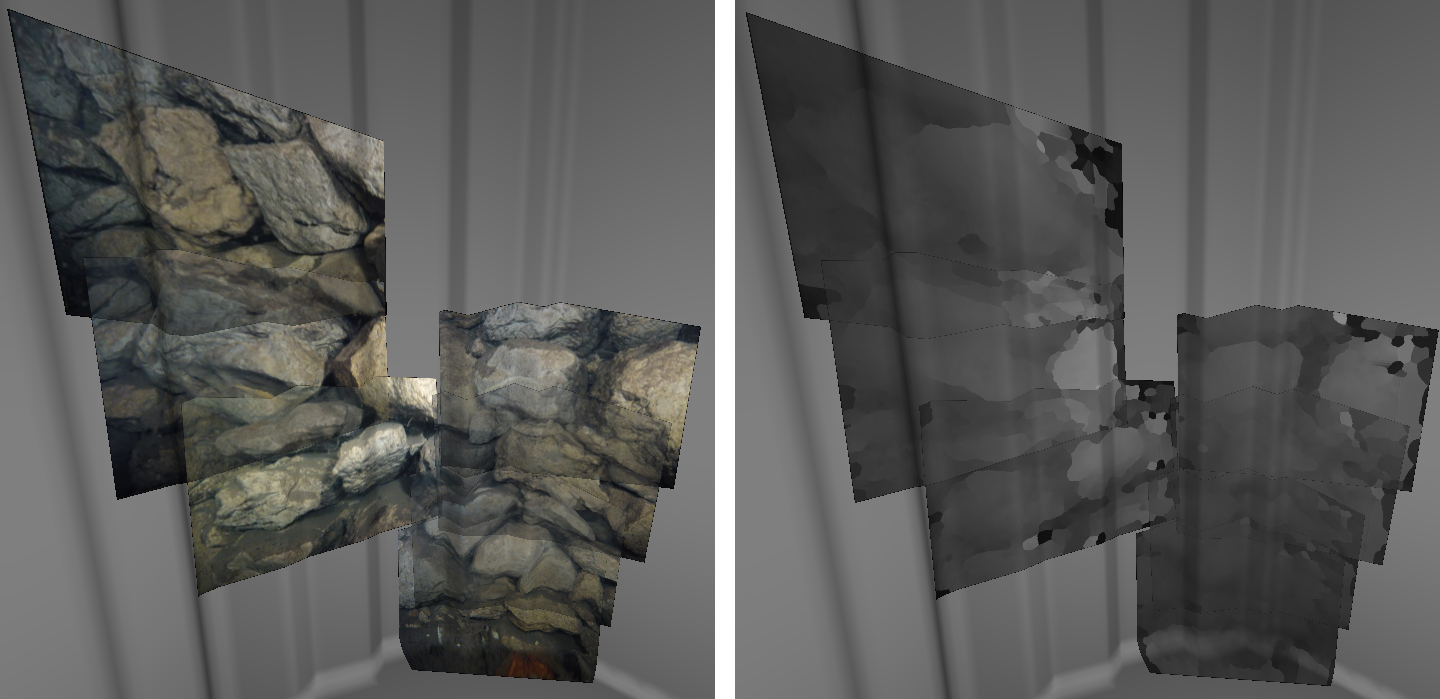
\epsfig{file = pics/NoDisplaceColorDisparity.png, width = 8cm}
	\caption{Images and disparity maps reprojected as they were captured inside the well with no vertex displacements.}
	\label{fig:result2}
\end{figure}

Finally, the disparity maps combined with the surface images were mapped into the well geometry to produce the detailed mesh in Figures~\ref{fig:result4} \&~\ref{fig:resultFull}. In our current implementation all textures are stored on the GPU, which limits the number we can currently display to X. Future work will include methods to cycle through textures.
%he only factor that is keeping us from filling the well with textures is the Glew texture limit. ???
%ZJW: really???  we need a way around that - Once you've displaced and colored vertices can't you release a texture and cycle through more? - the above sounds fairly weak....

%need to figure out how to do a gradient fade between wireframe and real images
%\begin{figure}[!h]
%	\vspace{-0.2cm}
%	\centering
%		\epsfig{file = pics/400kUpClose2.png, width = 7cm}
%	\caption{Close view of displaced and textured geometry.}
%	\label{fig:result4}
%\end{figure}

%\begin{figure*}[!ht]
%   \vspace{-0.2cm}
%   \centering{
%      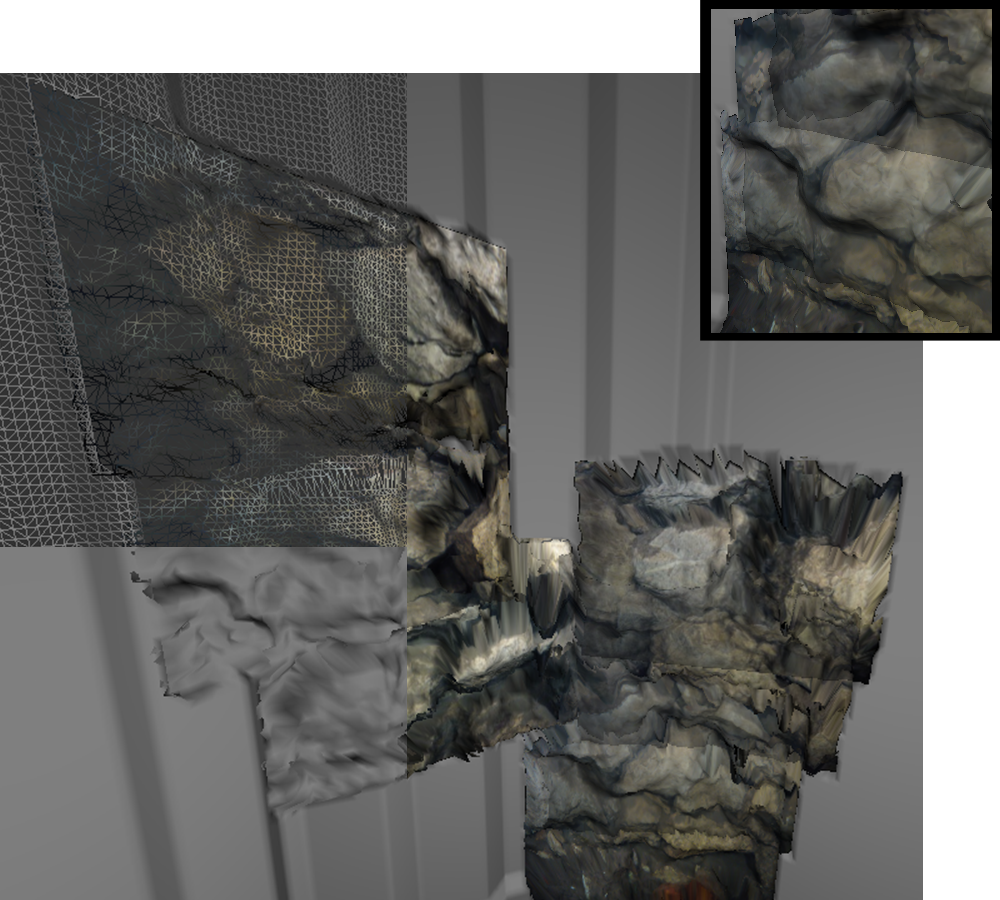
\epsfig{file = pics/400Composite2.png, width = .9\textwidth}}
%   \caption{View of depth and color data mapped onto part of the general mesh.. The fine details added by the vertex displacements and recalculated lighting create a better appearance of the walls of the well (including inset close-up view).}
%  \label{fig:resultFull}
%\end{figure*}

\begin{figure*}[!ht]
    \vspace{-0.2cm}
	\centering
		\subfigure[Full view]{\label{fig:composite}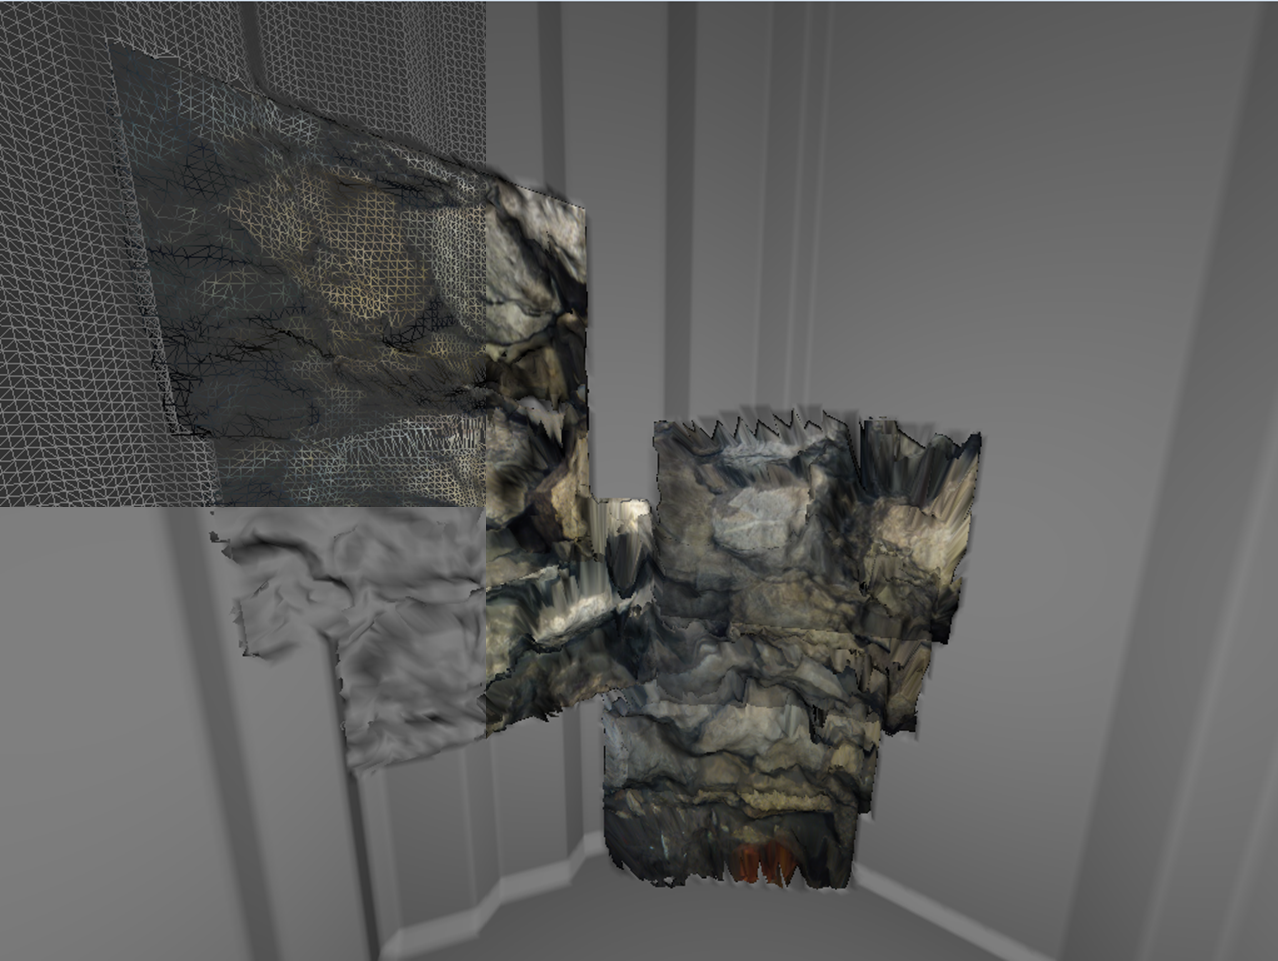
\epsfig{file = pics/400kCompositePic.png, width = 0.55\textwidth}}
		\quad %space between images
		\subfigure[Close view]{\label{fig:upclose}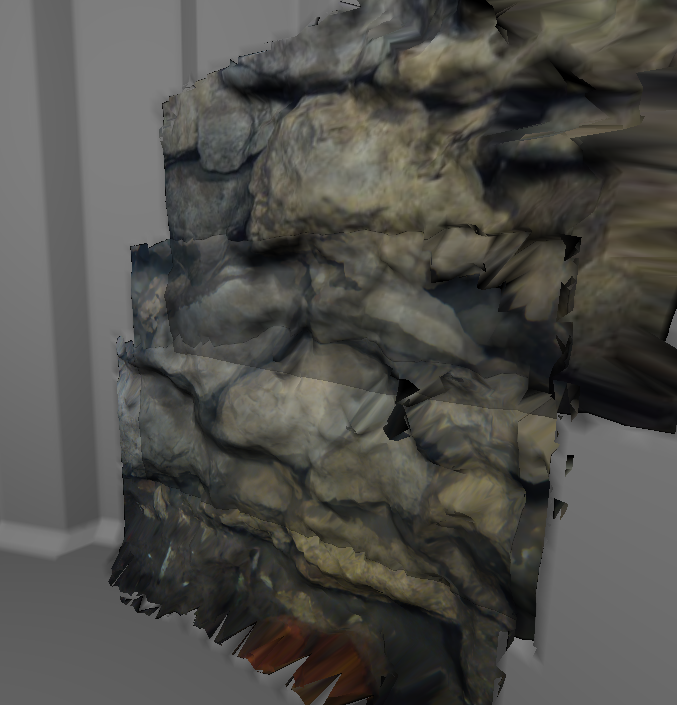
\epsfig{file = pics/400kUpClose.png, width = 0.3965\textwidth}}
		\caption{View of depth and color data mapped onto part of the general mesh.. The fine details added by the vertex displacements and recalculated lighting create a better appearance of the walls of the well.}
		\label{fig:resultFull}
\end{figure*}

\section{Conclusion and Future Work}
\label{sec:conclusion}
\noindent 
This paper presents a method of adding geometric details to maps created to represent underwater environments. 
%A general model is acquired from sonar data and mapping~\cite{ICEX11,McVicker,McVicker2}, and we present the addition of fine level details using stereo image data.  
This work is motivated by the desire to better map underwater caverns and cisterns using robotic tools.  We have presented our methodology and hardware for data acquisition, disparity map generation, and incorporation of that disparity data via projective texturing displacements.  We have shown results of a partial reconstruction of a well in Carini, Sicily.

In this preliminary work, we have discovered many of the key factors for obtaining more complete models and details.  Future enhancements include: the use of higher quality cameras, inclusion of color and more powerful lighting, addition of smart tether for better localization, and enhancement of memory management to process more textures and disparity maps at once.
%For example, more detailed disparity maps could be achieved by upgrading the cameras and the lights on the robot.

Additional lessons learned include: since the clearest pictures were taken before the ROV had uplifted sediment from the cistern floor by landing, the ROV should capture all images of the cistern wall before landing to record sonar scans. In the future, we would like to explore algorithms from texture synthesis and apply learning to a small subset of disparity images in order to generalize the small detailed geometry without having to acquire disparity maps of the entire wall (since complete data coverage is a challenge).

In addition, GoPro cameras were a simple, cost-effective, solution to acquire underwater stereo images.
With better cameras the output images would not need to be processed down to remove jpeg compression artifacts, which would allow much larger disparity images.  
Similarly, with better cameras there would be no need to compensate for different exposure times between images, and images could be captured synchronously.
Alternatively, better lighting, including blue lights, would allow pixel values to be compared in the HSL color space.
Such lighting additions could reduce the need for a different camera setup.  Finally, it would be interesting to explore the possibility of integrating this algorithm with a SLAM algorithm and more computing power to allow a robot to autonomously image each surface of a cistern. 

%Data collection in future deployments should be performed during a dry weather, as flowing rainwater dirtied the water and reduced image quality for the current data. 




%Unfortunately, that would require a far more complex setup that what we had available at the time of writing.

%ZJW: Please add some suggestion for actual data collection methods as well - re: lighting, positioning ROV, etc.
\begin{thebibliography}{9}
\bibitem{Clark2008b}
Clark, C.~M., Olstad, C., Buhagiar, K., and Gambin, T. (2008).
\newblock Archaeology via underwater robots: Mapping and localization within
  maltese cistern systems.
\newblock In {\em Proc. of the 10th International Conference on Control,
  Automation, Robotics and Vision (ICARCV 08).}

\bibitem{Fairfield:2010}
Fairfield, N., Kantor, G., Jonak, D., and Wettergreen, D. (2010).
\newblock Autonomous exploration and mapping of flooded sinkholes.
\newblock {\em Int. J. Rob. Res.}, 29(6):748--774.

\bibitem{Fairfield2005}
Fairfield, N., Kantor, G., and Wettergreen, D. (2005)).
\newblock Three dimensional evidence grids for {SLAM} in complex underwater
  environments.
\newblock In {\em Proceedings of the 14th International Symposium of Unmanned
  Untethered Submersible Technology (UUST).}

\bibitem{Fairfield2006}
Fairfield, N., Kantor, G., and Wettergreen, D. (2006)).
\newblock Real-time {SLAM} with octree evidence grids for exploration in
  underwater tunnels.
\newblock In {\em Journal of Field Robotics, Vol 24, Issue 1-2, pp. 03-21.}

\bibitem{ICEX11}
Forney, C., Forrester, J., Bagley, B., McVicker, W., White, J., Smith, T.,
  Batryn, J., Gonzalez, A., Lehr, J., Gambin, T., Clark, C.~M., and Wood, Z.~J.
  (2011).
\newblock Surface reconstruction of maltese cisterns using rov sonar data for
  archeological study.
\newblock In {\em Proceedings of the 7th international conference on Advances
  in visual computing - Volume Part I}, ISVC'11, pages 461--471, Berlin,
  Heidelberg. Springer-Verlag.

\bibitem{harbor}
Hern�ndez, E., Ridao, P., Ribas, D., and Batlle, J. (2009).
\newblock Msispic: A probabilistic scan matching algorithm using a mechanical
  scanned imaging sonar.
\newblock In {\em Journal of Physical Agents 3:3�11}.

\bibitem{ClarkVast}
Hiranandani, D., White, C., Clark, C., Gambin, T., and Buhagiar, K. (2009).
\newblock Underwater robots with sonar and smart tether for underground cistern
  mapping and exploration.
\newblock In {\em The 10th International Symposium on Virtual Reality,
  Archaeology and Cultural Heritage VAST}.

\bibitem{Lorensen}
Lorensen, W.~E. and Cline, H.~E. (1987).
\newblock Marching cubes: A high resolution {3D} surface construction
  algorithm.
\newblock In {\em Proceedings of the 14th Annual Conference on Computer
  Graphics and interactive Techniques}, pages 163--169.

\bibitem{McVicker}
McVicker, W., Forrester, J., Nelson, E., Gambin, T., Lehr, J., Wood, Z., and
  Clark, C. (2012).
\newblock Mapping and visualizing ancient water storage systems with an rov -
  an approach based on fusing stationary scans within a particle filter.

\bibitem{stereo:nalGast}
Nalpantidis, L. and Gasteratos, A. (2009).
\newblock Stereo vision for robotic applications in the presence of non-ideal
  lighting conditions.
\newblock (28).

\bibitem{opizarro-2009a}
Pizarro, O., Eustice, R.~M., and Singh, H. (2009).
\newblock Large area {3D} reconstructions from underwater optical surveys.
\newblock {\em IEEE Journal of Oceanic Engineering}.
\newblock In Press.

\bibitem{Segal}
Segal, M., Korobkin, C., van Widenfelt, R., Foran, J., and Haeberli, P. (1992).
\newblock Fast shadows and lighting effects using texture mapping.
\newblock In {\em In Computer Graphics (SIGGRAPH �92 Proceedings)}.

\bibitem{Thrun2005}
Thrun, S., Burgard, W., and Fox, D. (2005)).
\newblock Probabilistic robotics.
\newblock In {\em MIT Press.}

\bibitem{White10}
White, C., Hiranandani, D., Olstad, C., Buhagiar, K., Gabmin, T., and Clark, C.
  (2010).
\newblock The malta cistern mapping project: Underwater robot mapping and
  localization within ancient tunnel systems.
\newblock In {\em Journal of Field Robotics}.

\bibitem{Williams78castingcurved}
Williams, L. (1978).
\newblock Casting curved shadows on curved surfaces.
\newblock In {\em In Computer Graphics (SIGGRAPH �78 Proceedings}, pages
  270--274.

\bibitem{Williams2000}
Williams, S., Newman, P., Dissanayake, G., and Durrant-Whyte, H. (2000)).
\newblock Autonomous underwater simultaneous localization and map building.
\newblock In {\em Proceedings of the 2000 IEEE International Conference.}

\bibitem{Williams09}
Williams, S.~B., Pizarro, O., Jakuba, M., and Barrett, N. (2009).
\newblock {AUV} benthic habitat mapping in {S}outh {E}astern {T}asmania.
\newblock In {\em 7th InternationalConference on Field and Service Robotics}.

\bibitem{stereo:zitKan}
Zitnick, L. and Kanade, T. (1999).
\newblock A cooperative algorithm for stereo matching and occlusion detection.
\end{thebibliography}
\end{document}
